\newcommand\DP{\delta p}
\newcommand\dd{\mathrm{d}}
\newcommand\ul{\underline}

\section{Formulation par éléments finis --- Cas 1D}

Dans cette partie, l'objectif est d'exprimer le problème de la propagation acoustique dans une cavité unidimensionnelle
en utilisant le formalisme "éléments finis".

Le schéma du problème est présenté en figure~\ref{fig:FEM:propa_1D}.

\begin{figure}[!ht]
	\centering
	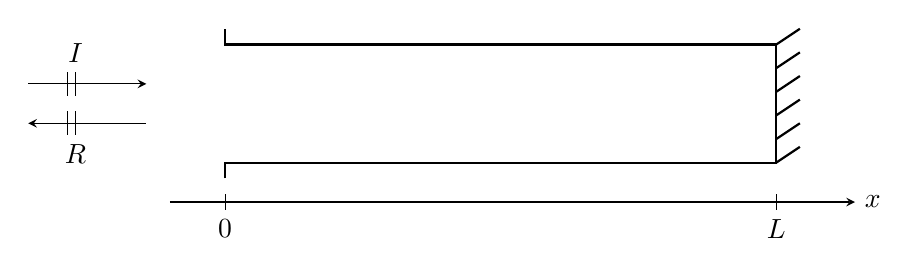
\begin{tikzpicture}[>=stealth]

	% waveguide
	\draw[thick] (0,.3) -- (0,.5) -- (7,.5) -- (7,2) -- (0,2) -- (0,2.2);
	\foreach \i in {0,...,5}{
		\draw[thick] (7,\i*0.3+0.5) -- ++(.3,.2);
	}
	
	% x axis
	\draw[->] (-.7,0) -- (8,0) node[right] {$x$};
	\draw (0,.1) -- ++(0,-.2) node[below] {$0$};
	\draw (7,.1) -- ++(0,-.2) node[below] {$L$};

	% waves
	% R
	\draw[<-] (-2.5,1) -- ++(1.5,0);
	\draw (-2,1.15) -- ++(0,-.3);
	\draw (-1.9,1.15) -- ++(0,-.3) node[below] {$R$};

	% I
	\draw[->] (-2.5,1.5) -- ++(1.5,0);
	\draw (-2,1.65) -- ++(0,-.3);
	\draw (-1.9,1.65) node[above] {$I$} -- ++(0,-.3);

\end{tikzpicture}


	\caption{\label{fig:FEM:propa_1D}Schéma du problème de propagation dans une cavité acoustique 1D de longueur L.}
\end{figure}

\paragraph{Position du Problème}

Le domaine considéré est noté $\Omega$ et sa frontière $\partial\Omega$.

Les conditions aux limites en $x=0$ et $x=L$ imposent :

\begin{equation}
	\left\{\begin{array}{l}
	\left.\partial_np\right|_{x=L} = 0\\
	\left.p\right|_{x=0} = p_i+p_r
	\end{array}\right. \label{FEM1D:BC}
\end{equation}


\paragraph{Formulation Variationnelle}

Le problème est régi par l'équation d'Helmholtz sans source telle que présentée en~\eqref{FEM1D:helm} (avec $k =
\nicefrac{\omega}{c}$ le nombre d'onde, $c$ la célérité du son dans le milieu, et $\omega$ la pulsation).

\begin{equation}
	(\Delta + k^2)p(x,\omega) = 0 \label{FEM1D:helm}
\end{equation}

En faisant usage de la formulation variationnelle (avec $\DP$ le champ variationnel), puis d'une intégration par
parties, le problème s'exprime comme en~\eqref{FEM1D:IPP}.

\begin{eqnarray}
	\int_\Omega \Delta p~\DP~\dd\Omega + k^2 \int_\Omega p~\DP~\dd\Omega & =  & 0,\quad \forall\DP\notag\\
	\int_\Omega p''~\DP~\dd\Omega + k^2 \int_\Omega p~\DP~\dd\Omega & =  & 0,\quad \forall\DP\notag\\
	\bigg[p'~\DP\bigg]_{\partial\Omega} - \int_\Omega p'~\DP' ~\dd\Omega + k^2\int_\Omega p~\DP~\dd\Omega & = & 0, \quad \forall\DP \label{FEM1D:IPP}
\end{eqnarray}

Considérant les conditions aux limites, il est possible de simplifier le crochet comme suit.

\begin{equation}
	\bigg[p'~\DP\bigg]_{\partial\Omega} = \underbrace{p'(L)\DP(L)}_{=0~\because~\left.\partial_np\right|_{x=L}= 0} - p'(0)\DP(0) \label{FEM1D:crochet}\\
\end{equation}

En ré-injectant~\eqref{FEM1D:crochet} dans~\eqref{FEM1D:IPP} et en ré-organisant les termes, il apparait l'équation~\ref{FEM1D:pre_vect}.

\begin{equation}
	\int_\Omega p'~\DP'~\dd\Omega - k^2\int_\Omega p~\DP~\dd\Omega = -p'(0)\DP(0), \quad \forall\DP \label{FEM1D:IPP}
\end{equation}

\paragraph{Fonctions de forme}

Supposant que les champs $p$ et $\DP$ sur un intervale $[x_i, x_j]$ sont décomposables en une combinaison linéaire de
fonctions $\phi_k$ (dites fonctions de forme) assorties des valeurs du champs aux extrémités du domaine, il vient :

\begin{equation}
	\left\{\begin{array}{l}
		p = \phi_1(x)p(x_i) + \phi_2(x)p(x_j)\\
		p' = \phi_1'(x)p_i + \phi_2'(x)p(x_j)\\
	\end{array}\right., \quad
	\left\{\begin{array}{l}
		\DP = \phi_1(x)\DP(x_i) + \phi_2(x)\DP(x_j)\\
		\DP' = \phi_1'(x)\DP(x_i) + \phi_2'(x)\DP(x_j)\\
	\end{array}\right.\label{FEM1D:shapefun}
\end{equation}

Pour alléger les notations, on pose $\alpha_k\equiv \alpha(x_k)$ où $\alpha$ est un champ et $x_k$ un point, de même
$\phi_k\equiv\phi_k(x)$.
Il est alors possible de ré-écrire les équations de~\eqref{FEM1D:shapefun} de manière vectorielle comme présenté
en~\eqref{FEM1D:shapevec}.

\begin{equation}
	\left\{\begin{array}{l}
		p = \big[\phi_1\big|\phi_2\big]\begin{Bmatrix}p_i\\p_j\end{Bmatrix}\\
		p' = \big[\phi_1'\big|\phi_2'\big]\begin{Bmatrix}p_i\\p_j\end{Bmatrix}\\
	\end{array}\right.,\quad
	\left\{\begin{array}{l}
		\DP = \big[\phi_1\big|\phi_2\big]\begin{Bmatrix}\DP_i\\\DP_j\end{Bmatrix}\\
		\DP' = \big[\phi_1'\big|\phi_2'\big]\begin{Bmatrix}\DP_i\\\DP_j\end{Bmatrix}\\
	\end{array}\right.\label{FEM1D:shapevec}
\end{equation}

En utilisant cette dernière équation~\eqref{FEM1D:shapevec}, en considérant une partition du domaine $\Omega$ de sorte
que $\Omega = \sum_e\Omega_e$ où l'équation~\eqref{FEM1D:helm} est vérifiée sur chacune des parties de $\Omega$ et en
utilisant la relation de Chasles, il vient :

\begin{equation}
	\int_\Omega p'~\DP'~\dd\Omega - k^2\int_\Omega p~\DP~\dd\Omega = -p'(0)\DP(0) = 
		\sum_e \left\{\int_{\Omega_e} p'~\DP'~\dd\Omega - k^2\int_{\Omega_e} p~\DP~\dd\Omega \right\}= -p'(0)\DP(0), \quad \forall\DP \label{FEM1D:IPP}
\end{equation}
